% Options for packages loaded elsewhere
\PassOptionsToPackage{unicode}{hyperref}
\PassOptionsToPackage{hyphens}{url}
%
\documentclass[
]{article}
\title{Ejercicio 3. Tarea 2: Consumo. Macroeconomía}
\author{Benjamín Elam Rodríguez Alcaraz}
\date{3/9/2022}

\usepackage{amsmath,amssymb}
\usepackage{lmodern}
\usepackage{iftex}
\ifPDFTeX
  \usepackage[T1]{fontenc}
  \usepackage[utf8]{inputenc}
  \usepackage{textcomp} % provide euro and other symbols
\else % if luatex or xetex
  \usepackage{unicode-math}
  \defaultfontfeatures{Scale=MatchLowercase}
  \defaultfontfeatures[\rmfamily]{Ligatures=TeX,Scale=1}
\fi
% Use upquote if available, for straight quotes in verbatim environments
\IfFileExists{upquote.sty}{\usepackage{upquote}}{}
\IfFileExists{microtype.sty}{% use microtype if available
  \usepackage[]{microtype}
  \UseMicrotypeSet[protrusion]{basicmath} % disable protrusion for tt fonts
}{}
\makeatletter
\@ifundefined{KOMAClassName}{% if non-KOMA class
  \IfFileExists{parskip.sty}{%
    \usepackage{parskip}
  }{% else
    \setlength{\parindent}{0pt}
    \setlength{\parskip}{6pt plus 2pt minus 1pt}}
}{% if KOMA class
  \KOMAoptions{parskip=half}}
\makeatother
\usepackage{xcolor}
\IfFileExists{xurl.sty}{\usepackage{xurl}}{} % add URL line breaks if available
\IfFileExists{bookmark.sty}{\usepackage{bookmark}}{\usepackage{hyperref}}
\hypersetup{
  pdftitle={Ejercicio 3. Tarea 2: Consumo. Macroeconomía},
  pdfauthor={Benjamín Elam Rodríguez Alcaraz},
  hidelinks,
  pdfcreator={LaTeX via pandoc}}
\urlstyle{same} % disable monospaced font for URLs
\usepackage[margin=1in]{geometry}
\usepackage{longtable,booktabs,array}
\usepackage{calc} % for calculating minipage widths
% Correct order of tables after \paragraph or \subparagraph
\usepackage{etoolbox}
\makeatletter
\patchcmd\longtable{\par}{\if@noskipsec\mbox{}\fi\par}{}{}
\makeatother
% Allow footnotes in longtable head/foot
\IfFileExists{footnotehyper.sty}{\usepackage{footnotehyper}}{\usepackage{footnote}}
\makesavenoteenv{longtable}
\usepackage{graphicx}
\makeatletter
\def\maxwidth{\ifdim\Gin@nat@width>\linewidth\linewidth\else\Gin@nat@width\fi}
\def\maxheight{\ifdim\Gin@nat@height>\textheight\textheight\else\Gin@nat@height\fi}
\makeatother
% Scale images if necessary, so that they will not overflow the page
% margins by default, and it is still possible to overwrite the defaults
% using explicit options in \includegraphics[width, height, ...]{}
\setkeys{Gin}{width=\maxwidth,height=\maxheight,keepaspectratio}
% Set default figure placement to htbp
\makeatletter
\def\fps@figure{htbp}
\makeatother
\setlength{\emergencystretch}{3em} % prevent overfull lines
\providecommand{\tightlist}{%
  \setlength{\itemsep}{0pt}\setlength{\parskip}{0pt}}
\setcounter{secnumdepth}{-\maxdimen} % remove section numbering
\ifLuaTeX
  \usepackage{selnolig}  % disable illegal ligatures
\fi

\begin{document}
\maketitle

\hypertarget{ejercicio-3.-estudie-el-consumo-agregado-en-muxe9xico-siguiendo-estos-pasos-3-horas-0.5-puntos-cada-inciso}{%
\subsection{Ejercicio 3. Estudie el consumo agregado en México siguiendo
estos pasos: {[}3 horas, 0.5 puntos cada
inciso{]}}\label{ejercicio-3.-estudie-el-consumo-agregado-en-muxe9xico-siguiendo-estos-pasos-3-horas-0.5-puntos-cada-inciso}}

\hypertarget{a-obtenga-del-inegi-datos-de-c-el-consumo-agregado-en-muxe9xico-de-y-elproducto-agregado-de-i-la-inversiuxf3n-agregada-de-g-el-gasto-del-gobierno-y-de-de-nx-las-exportaciones-netas-entre-1980-y-el-tercer-trimestre-de-2019en-tuxe9rminos-reales}{%
\subsubsection{a) Obtenga, del Inegi, datos de ``C'', el consumo
agregado en México, de ``Y'', elproducto agregado, de ``I'', la
inversión agregada, de ``G'', el gasto del gobierno y de , de ``NX'',
las exportaciones netas, entre 1980 y el tercer trimestre de 2019,EN
TÉRMINOS
REALES}\label{a-obtenga-del-inegi-datos-de-c-el-consumo-agregado-en-muxe9xico-de-y-elproducto-agregado-de-i-la-inversiuxf3n-agregada-de-g-el-gasto-del-gobierno-y-de-de-nx-las-exportaciones-netas-entre-1980-y-el-tercer-trimestre-de-2019en-tuxe9rminos-reales}}

Se obtuvieron las siguientes series:

\begin{itemize}
\tightlist
\item
  Serie desestacionalizada: Indicador Mensual del Consumo Privado en el
  Mercado Interior (en adelante ``C'') de base 2013 \footnote{Vale la
    pena hacer la siguiente aclaración: la series disponibles en INEGI
    son del periodo 1993-2021. El ejercicio pide desde el año 1980, pero
    algunas series disponibles en la estadístia oficial datan de 1993
    dado que, a partir de 1994 se homologaron metodologías estadísticas
    entre los países parte del \emph{TMEC} y se ajustaron a base
    2013=100, por lo que la búsqueda de datos anteriores a esta
    homologación podría resultar difícil para trabajar y significaría un
    trabajo estadístico de datos (para hacer las series comparables) que
    excede los propósitos de esta tarea, por lo que las series se
    tomaron para todo el periodo disponible, a reserva de que la
    tendencia, básicamente, se mantiene y las conclusiones que podemos
    sacar del análisis no variarían significativamente.}.
\end{itemize}

\begin{itemize}
\tightlist
\item
  Serie desestacionalizada: Producto Interno Bruto (en adelante ``Y'') a
  precios 2013.
\item
  Serie desestacionalizada: Inversión Bruta Fija (en adelante ``I'') de
  base 2013.
\item
  Serie desestacionalizada: Gasto programable (en adelante ``G'') a
  precios 2013 \footnote{Esta serie se desestacionalizó aparte, dado que
    fue descargada en niveles de Banxico. El Gasto se divide en gasto de
    capital y gasto corriente. Decidimos tomar el gasto programable ya
    que es el que se planea ejercer en el presupuesto de cada año,
    aunque, además, hay un gasto no programable, que es aquel que se
    ejerce y que no estaba presupuestado.}.
\item
  Serie desestacionalizada: Balanza comercial (en adelante ``XN'') a
  precios 2013 \footnote{Íbidem.}.
\end{itemize}

Ahora, para obtener las series en términos reales, las deflactamos con
el INPC. Esto se hace solamente con las variables \(G\) y \(XN\) ya que
éstas son variables en niveles. De aquí en adelante, las series se
presentan en términos reales, desestacionalizadas y de base 2013.

Aprovecharemos, en este inciso, para mostrar el proceso por el cual se
desestacionalizó la variable \(G\) así como \(XN\). Lo primero es
identificar que toda serie de tiempo tiene 4 componentes, a saber:
ciclo, tendencia, estacionalidad e irregularidad. Se descompuso la serie
en sus 4 componentes, que para el caso de \(G\) se observan a
continuación:

\begin{figure}
\centering
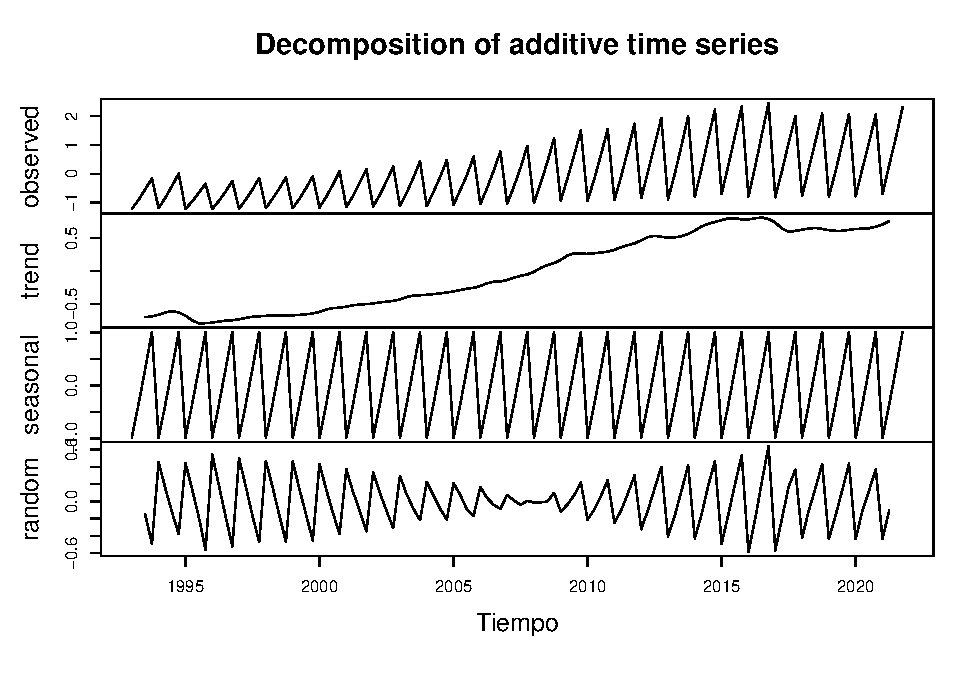
\includegraphics{Ejercicio-3_files/figure-latex/unnamed-chunk-2-1.pdf}
\caption{Descomposición de la serie G}
\end{figure}

De esta descomposición solamente obtenemos el componente de la tendencia
para la variable \(G\). Lo mismo sucede para la variable \(XN\).

Las series que se trabajarán a lo largo de este ejercicio son las que
siguen:

\begin{figure}
\centering
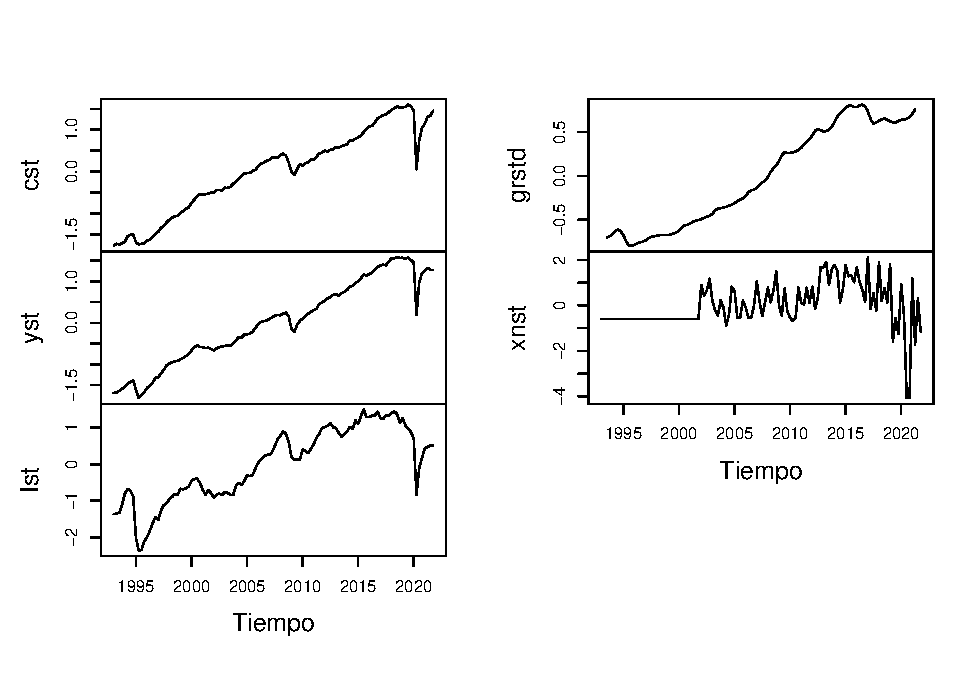
\includegraphics{Ejercicio-3_files/figure-latex/unnamed-chunk-3-1.pdf}
\caption{Variables macroeconómicas seleccionadas}
\end{figure}

Nótese que las variables están suavizadas y normalizadas, así como están
en términos reales a precios 2013. Notemos que la variación y la
tendencia entre las variables \(Y_t\), \(I_t\) y \(C_t\) es muy similar,
lo que indica que hay un grado de asociación entre dichas variables muy
importante. Notemos que esto puede tener alguna implicación en los
resultados econométricos que se analizarán en el inciso f).

\hypertarget{b-grafique-dichas-serie-de-tiempo-juntas-para-comparalas-visualmente.-compare-la-gruxe1fica-de-las-variables-de-las-que-son-siempre-positivas-en-dos-versiones-asu-valor-real-original-y-b-despuuxe9s-de-sacarles-el-logaritmo-natural.}{%
\subsubsection{b) Grafique dichas serie de tiempo juntas para comparalas
visualmente. (Compare la gráfica de las variables (de las que son
siempre positivas) en dos versiones: a)su valor real original, y b)
después de sacarles el logaritmo
natural).}\label{b-grafique-dichas-serie-de-tiempo-juntas-para-comparalas-visualmente.-compare-la-gruxe1fica-de-las-variables-de-las-que-son-siempre-positivas-en-dos-versiones-asu-valor-real-original-y-b-despuuxe9s-de-sacarles-el-logaritmo-natural.}}

\hypertarget{b.1-graficando-en-su-valor-original}{%
\paragraph{b.1) Graficando en su valor
original}\label{b.1-graficando-en-su-valor-original}}

Para realizar este inciso tuvimos que normalizar las variables para
hacerlas comparables, esto debido a que los valores máximos y mínimos de
estas son muy disímiles. La normalización se dio a través de la
siguiente fórmula:

\(Z_i=\frac{X_i- \mu}{\sigma}\)

Donde \(x_i\) es cada una de las observaciones de las series para cada
\(t_i\), con \(t_i \in[1993I-2021IV]\) lo que nos devolverá un nuevo
valor \(z_i\) para \(t_i\in[1993I-2021IV]\), de esta forma no se pierde
ninguna observación y sólo se modifica la escala, lo que nos permite
hacer comparaciones entre las variables. En la siguiente gráfica se
muestran las variables en niveles: \(C\), \(Y\), \(I\) y \(G\).

\begin{figure}
\centering
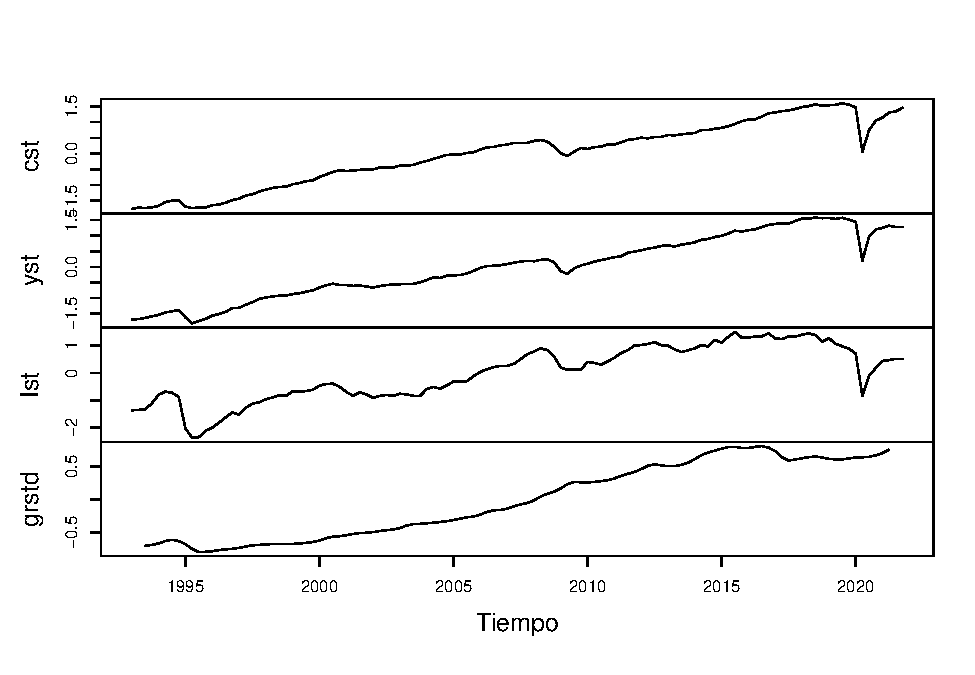
\includegraphics{Ejercicio-3_files/figure-latex/unnamed-chunk-4-1.pdf}
\caption{Variables seleccionadas: 1993-2022}
\end{figure}

Nótese que estas variables tienen un comportamiento similar. En todo el
periodo la tendencia es creciente, con una caída importante durante la
pandemia y a partir del Gobierno de Andrés Manuel López Obrador. Nótese,
además, que el \(G\) tuvo una caída menor, pues a partir de la crisis
económica generada por la pandemia el gobierno en turno incentivó la
economía a través de una política fiscal expansiva.

\hypertarget{b.2-graficando-su-ln}{%
\paragraph{b.2) Graficando su ln}\label{b.2-graficando-su-ln}}

Para realizar este inciso se tomaron los \(ln(x_i)\) donde \(x_i\) es
cada variable analizada. En este caso tenemos lo que sigue:
\(ln(c), ln(Y), ln(I)\) y \(ln(G)\) \footnote{Nótese que, para el caso
  de la variable \(ln(G)\), al normalizarla, los valores para el
  logaritmo natural son negativos, por lo que no se alcanzan a ver en la
  gráfica. No es sino hasta el tercer trimestre de 2009 que los valores
  son positivos y pueden compararse.}.

Notamos que el comportamiento tendencial de las variables se mantiene:
hay una tendencia creciente en el periodo con una variación negativa
durante los últimos años del periodo debido a las razones que ya
mencionamos.

\begin{figure}
\centering
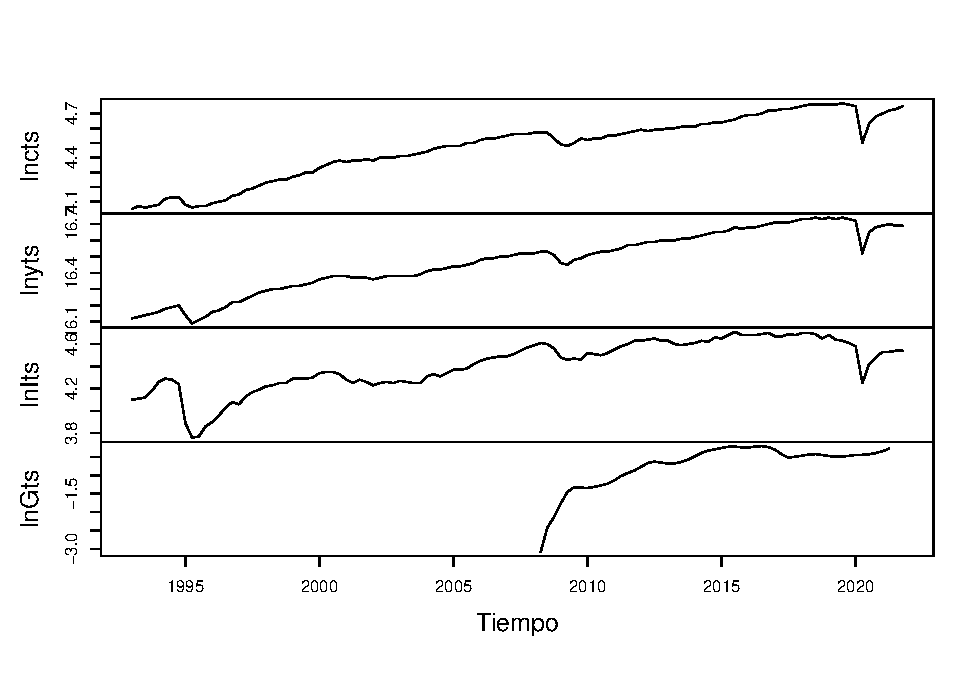
\includegraphics{Ejercicio-3_files/figure-latex/unnamed-chunk-6-1.pdf}
\caption{Variables seleccionadas en logaritmo: 1993-2022}
\end{figure}

\hypertarget{c-grafique-tambiuxe9n-la-tasa-de-crecimiento-de-todas-estas-series}{%
\subsubsection{c) Grafique también la tasa de crecimiento de todas estas
series}\label{c-grafique-tambiuxe9n-la-tasa-de-crecimiento-de-todas-estas-series}}

La tasa de crecimiento de cada una de las series está dada por la
siguiente ecuación:

\(\Delta{x_t}=(X_t - X_{t-1}) / X_{t-1} \times 100\)

Donde cada \(\Delta{x_t}\) es un valor para el tiempo \(t\) que medirá
la variación que tuvo cada observación respecto al tiempo \(t-1\). Este
valor está expresado en porcentaje.

En la siguiente gráfica observamos las variaciones de las variables
seleccionadas.

\begin{figure}
\centering
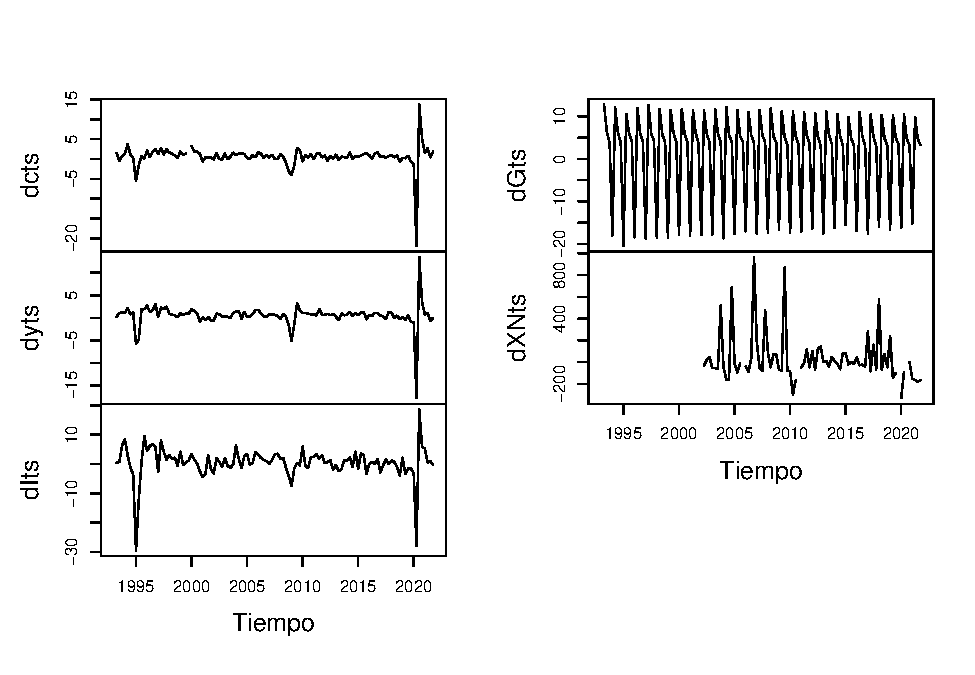
\includegraphics{Ejercicio-3_files/figure-latex/unnamed-chunk-8-1.pdf}
\caption{Variaciones porcentuales de variables seleccionadas: 1993-2022}
\end{figure}

Notemos que \(\Delta{C_t}\), \(\Delta{Y_t}\) y \(\Delta{I_t}\) son muy
similares, esto debido a la correlación que existe entre las variables.
Por otro lado, \(\Delta{G_t}\) y \(\Delta{XN_t}\) tienen una dinámica
distinta. Notemos, además, que \(\Delta{XN_t}\) es una serie que
decrece, pues México tiene una dinámica de déficit comercial, es decir,
que en México para \(t\in[2002-2021]\) se cumple que \(X_t \leq M_t\),
luego entonces, \(XN_t\leq0\). Véase también que, en el caso de
\(\Delta{G_t}\) las variaciones son muy altas, es decir, es más volatil.
Esto se explica porque el gasto programable varía en función de los
recursos disponibles del Gobierno en cada periodo \(t\) y, además, de
las proyecciones que se tienen respecto al comportamiento de las
variables clave que financian el \(G\). Estas variables son
,\emph{grosso modo}, el precio del petróleo y el índice de recaudación
fiscal.

\hypertarget{d-enfuxf3quese-ahora-nada-muxe1s-al-consumo-y-al-producto-agregado.-grafique-la-relaciuxf3n-entre-una-serie-y-la-otra-es-decir-grafique-los-puntos-deltay_t-deltac_t-poniendo-el-consumo-en-las-ordenadas}{%
\subsubsection{\texorpdfstring{d) Enfóquese ahora nada más al consumo y
al producto agregado. Grafique la relación entre una serie y la otra, es
decir, grafique los puntos (\(\Delta{Y_t}\), \(\Delta{C_t}\)) poniendo
el consumo en las
ordenadas}{d) Enfóquese ahora nada más al consumo y al producto agregado. Grafique la relación entre una serie y la otra, es decir, grafique los puntos (\textbackslash Delta\{Y\_t\}, \textbackslash Delta\{C\_t\}) poniendo el consumo en las ordenadas}}\label{d-enfuxf3quese-ahora-nada-muxe1s-al-consumo-y-al-producto-agregado.-grafique-la-relaciuxf3n-entre-una-serie-y-la-otra-es-decir-grafique-los-puntos-deltay_t-deltac_t-poniendo-el-consumo-en-las-ordenadas}}

Esta variación conjunta entre \(\Delta{C_t}\) y \(\Delta{Y_t}\) no es
clara si graficamos como la gráfica que sigue, sin embargo, nótese que
esta relación es positiva, es decir, intuitivamente podemos decir que
las variaciones positivas de \(Y_t\) se relacionan con variaciones
positivas de \(C_t\).

\begin{figure}
\centering
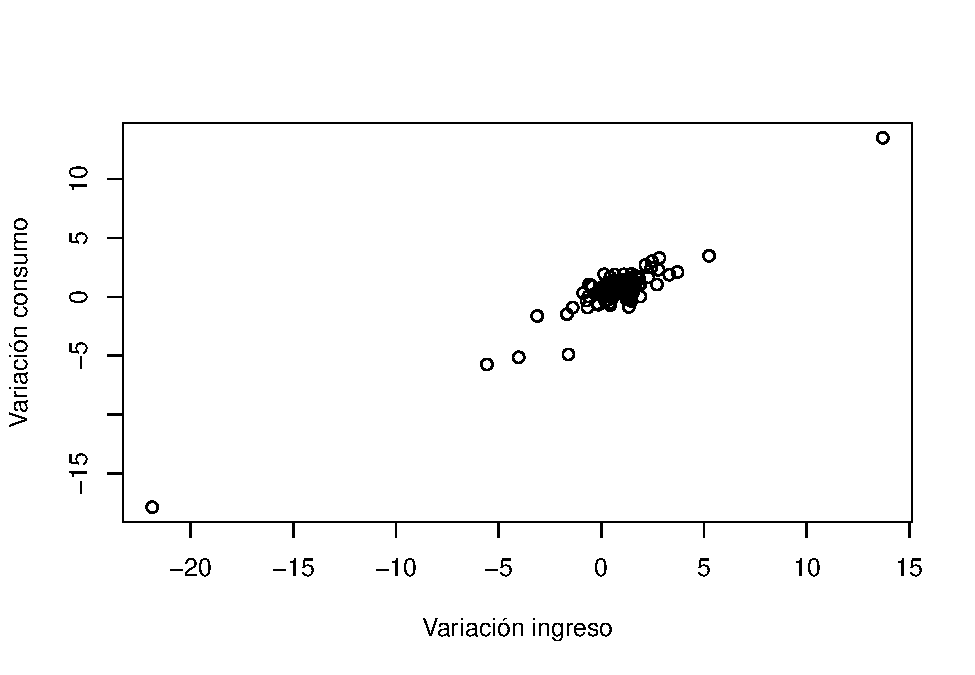
\includegraphics{Ejercicio-3_files/figure-latex/unnamed-chunk-9-1.pdf}
\caption{Relación entre \%Y y \%C}
\end{figure}

Notemos que esta relación es difícil de ver, dado que las variaciones
son muy disímiles. Hagamos ahora la comparación con las variables en
logaritmos. En la siguiente gráfica se muestra esta relación.

\begin{figure}
\centering
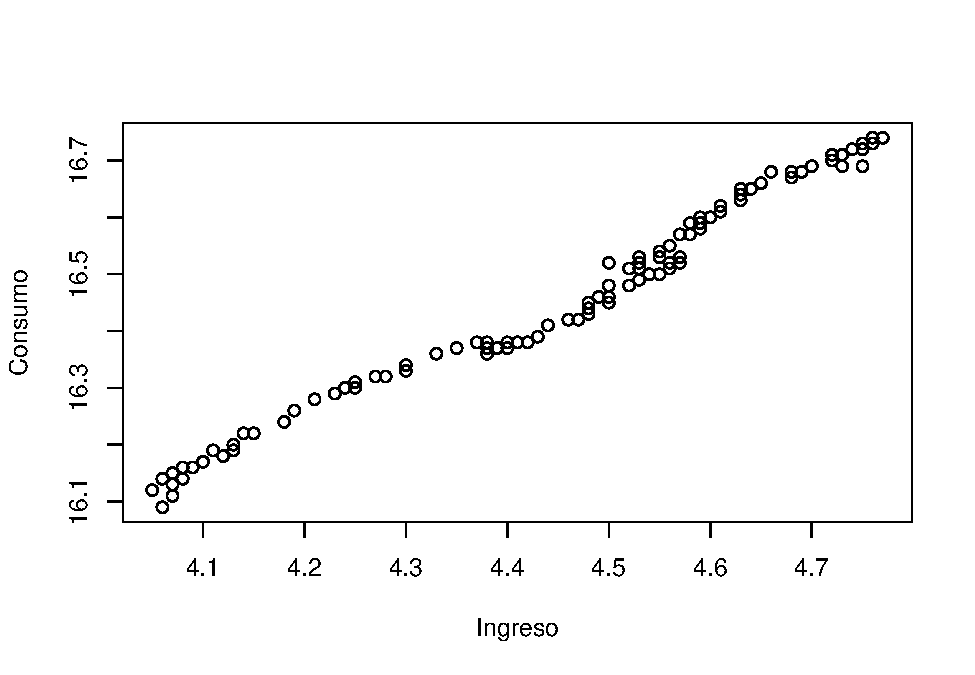
\includegraphics{Ejercicio-3_files/figure-latex/unnamed-chunk-10-1.pdf}
\caption{Relación entre ln(Y) y ln(C)}
\end{figure}

Nótese que esta relación es positiva, es decir, la variación del consumo
y del ingreso tiene un alto nivel de correlación. Esta relación nos
indica que el consumo crece conforme crece el ingreso, es decir, guardan
una relación directa \footnote{Notemos que esta es la relación que
  esperaríamos siguiendo la macroeconomía Keynesiana. Más adelante,
  estableceremos formal y econométricamente esta relación, buscando
  calcular la propensión marginal al consumo en el modelo 1 a estimar en
  el inciso f.~}.

\hypertarget{e-calcule-la-volatilidad-de-las-dos-series.-quuxe9-es-muxe1s-volatil-el-consumo-o-el-ingreso}{%
\subsubsection{e) Calcule la volatilidad de las dos series. ¿Qué es más
volatil, el consumo o el
ingreso?}\label{e-calcule-la-volatilidad-de-las-dos-series.-quuxe9-es-muxe1s-volatil-el-consumo-o-el-ingreso}}

Sabemos que la volatilidad de un conjunto de datos está dada por la raíz
cuadrada de la varianza, es decir, por la siguiente ecuación:

\(S_n=\sqrt{\sigma^2}\)

A su vez, sabemos que la varianza \(\sigma^2\) se define como sigue:

\(\sigma^2=\frac{1}{n}\sum(x_i-\mu)^2\)

Donde la varianza de \(C_t\) está dada por lo siguiente:

Notemos entonces que los datos son los siguientes:

\begin{equation}
\begin{bmatrix}
Varianza C & Varianza Y 
\end{bmatrix}
\end{equation}

\begin{center}
$=$
\end{center}

\begin{equation}
\begin{bmatrix}
321.896 & 251.7195
\end{bmatrix}
\end{equation}

Mientras que las desviaciones estándar están dadas por lo que sigue:

\begin{equation}
\begin{bmatrix}
Desviación C & Desviación Y 
\end{bmatrix}
\end{equation}

\begin{center}
$=$
\end{center}

\begin{equation}
\begin{bmatrix}
17.94 & 15.86
\end{bmatrix}
\end{equation}

Con esto podemos dar cuenta que es el consumo el que presenta una
variación ligeramente mayor y, por ende, es más volátil. Ahora, esto
puede deberse a que la variación en el ingreso está \emph{suavizada} por
las variaciones de los demás componentes, incluida la variación del
consumo.

\hypertarget{f-estimar-algunos-modelos-de-regresiuxf3n-lineal}{%
\subsubsection{f) Estimar algunos modelos de regresión
lineal:}\label{f-estimar-algunos-modelos-de-regresiuxf3n-lineal}}

Estimamos los siguientes modelos de regresión lineales:

\begin{itemize}
\tightlist
\item
  \(C_t=a + bY_t+\epsilon_t\)
\item
  \(\Delta_{C_t}=a+b\Delta_{Y_t}+\epsilon_t\)
\item
  \(\Delta_{C_t}=a+b\Delta_{Y_t-1}+\epsilon_t\)
\item
  \(ln(c_t)=a+bln(y_t)+\epsilon_t\)
\end{itemize}

\begin{enumerate}
\def\labelenumi{\arabic{enumi}.}
\tightlist
\item
  Los resultados para el primer modelo, \(C_t=a + bY_t+\epsilon_t\), se
  muestran a continuación:
\end{enumerate}

\(C_t=-000000.5+09.9Y_t\)

Es decir, que a cambios en \(Y_t\) el consumo responderá de forma
directa en un 9.9, lo que viene dado por el coeficiente \(b=09.9\).

Notemos que el valor para el intercepto es muy cercano a 0, por lo que
asumimos que \(a=0\).

Esta regresión se grafica en la siguiente tabla. Nótese que la relación
es directa y que el consumo está suficientemente explicado por el
ingreso.

Notemos que la propensión marginal a consumir es igual a 0.9, es decir,
que cambios en el ingreso se traducen casi proporcionalmente a cambios
en el consumo, siendo la diferencia, es decir, 0.1, la propensión
marginal a ahorrar.

\begin{figure}
\centering
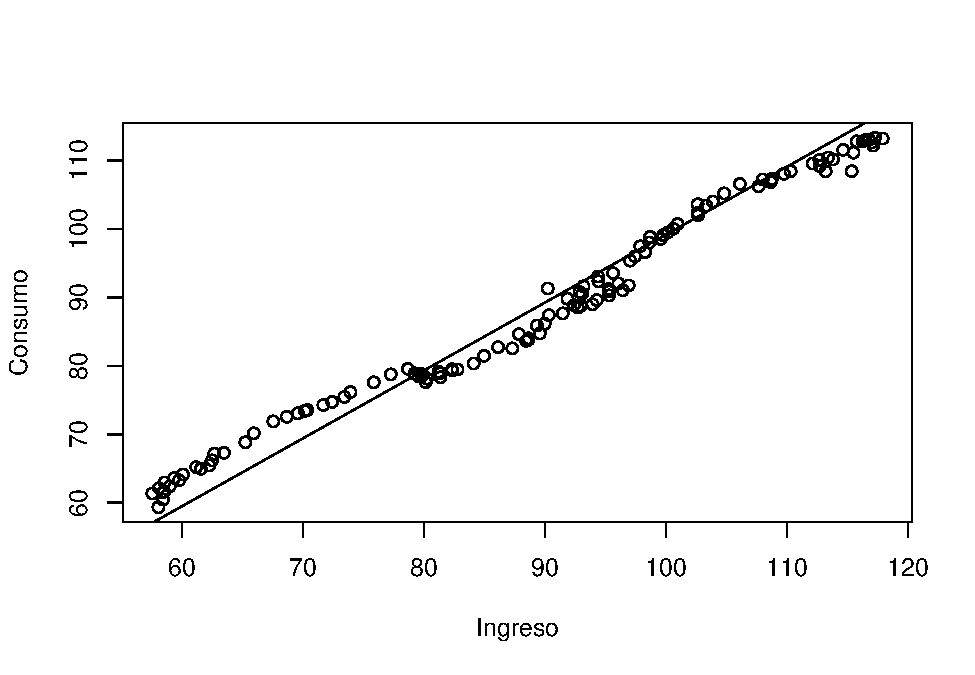
\includegraphics{Ejercicio-3_files/figure-latex/unnamed-chunk-12-1.pdf}
\caption{Modelo de regresión 1}
\end{figure}

Ahora notemos los errores. Eston están dados en la siguiente gráfica.
Notemos que estos errores presentan un patrón, lo que indica que hay
asociación lineal entre las variables. En el resumen de los estadísticos
de la regresión notaremos esta salvedad de la regresión:

\begin{figure}
\centering
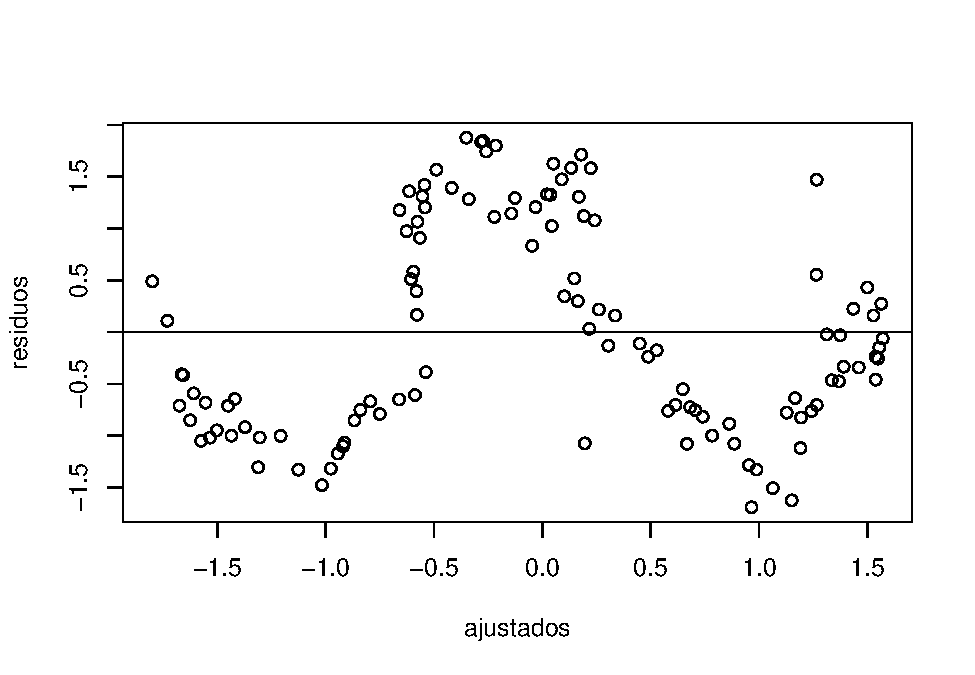
\includegraphics{Ejercicio-3_files/figure-latex/unnamed-chunk-13-1.pdf}
\caption{Errores: Modelo de regresión 1}
\end{figure}

La siguiente tabla muestra los resultados:

\textbackslash begin\{table\}\{h\} \textbackslash begin\{center\}
\textbackslash begin\{tabular\}\{\textbar l\textbar l\textbar c\textbar\}
\textbf{Coef.} \& \textbf{Estimado} \& \textbf{Std. Error} \&
\textbf{T\_value}\textbackslash{} \hline intercepto \& -5.510e-16 \&
00.1212 \& 0.00\textbackslash{} \hline Y \& 09.915 \& 00.1218 \&
81.42\textbackslash{} \hline R\^{}2 \& 0.9831 \& Adjusted R\^{}2 \&
0.9829\textbackslash{} \hline

\caption{Resultados}

\textbackslash end\{center\} \textbackslash end\{table\}

Notemos que la \(R^2\) ajustada es muy alta, es decir, que el consumo se
explica completamente por el ingreso. Como ya mencionamos, este
resultado indica que hay asociación lineal entre las variables pues la
\emph{bondad de ajuste} es cercana al 100\%.

\begin{enumerate}
\def\labelenumi{\arabic{enumi}.}
\setcounter{enumi}{1}
\tightlist
\item
  Ahora estimemos el segundo modelo de regresión lineal, de acuerdo con
  la ecuación que sigue:
\end{enumerate}

\(\Delta_{C_T}=a+b\Delta_{Y_t}+\epsilon_t\)

Los resultados se muestran a continuación:

\(\Delta_C=4.30+0.8\Delta_y\)

Esta regresión se grafica en la siguiente tabla. Nótese que la relación
es directa y que las variaciones en el consumo están suficientemente
explicadas por las variaciones en el ingreso.

Notemos que la propensión marginal a consumir es igual a 0.8, es decir,
que cambios en el ingreso se traducen casi proporcionalmente a cambios
en el consumo, siendo la diferencia, es decir, 0.2, la propensión
marginal a ahorrar.

\begin{figure}
\centering
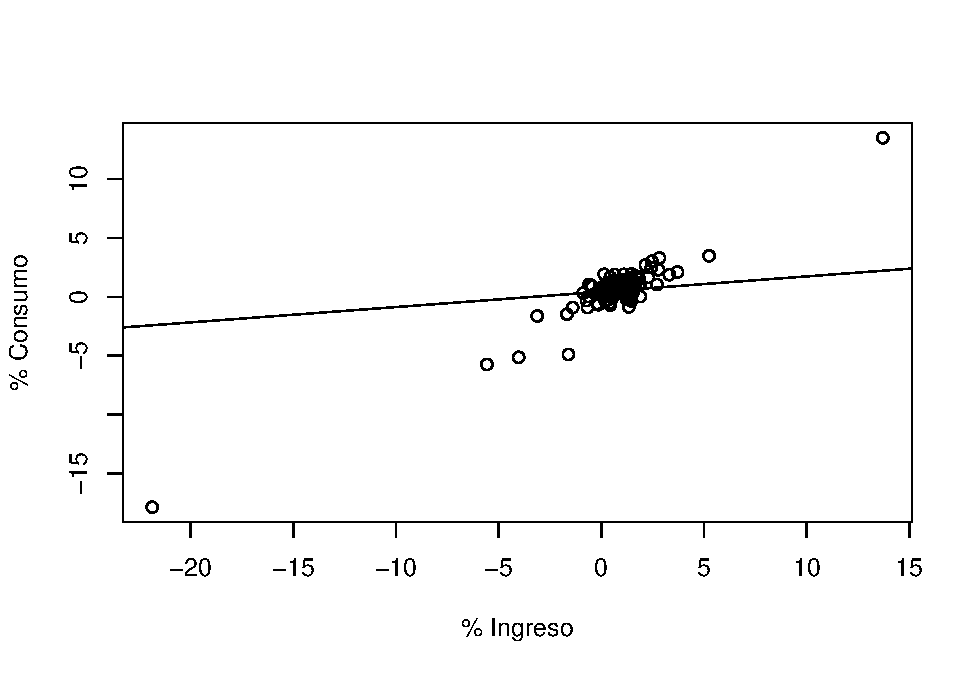
\includegraphics{Ejercicio-3_files/figure-latex/unnamed-chunk-14-1.pdf}
\caption{Modelo de regresión 2}
\end{figure}

Ahora notemos los errores. Eston están dados en la siguiente gráfica.
Notemos que estos errores no se distribuyen aleatoriamente, lo que
indica que hay asociación lineal entre las variables. En el resumen de
los estadísticos de la regresión notaremos esta salvedad de la
regresión.

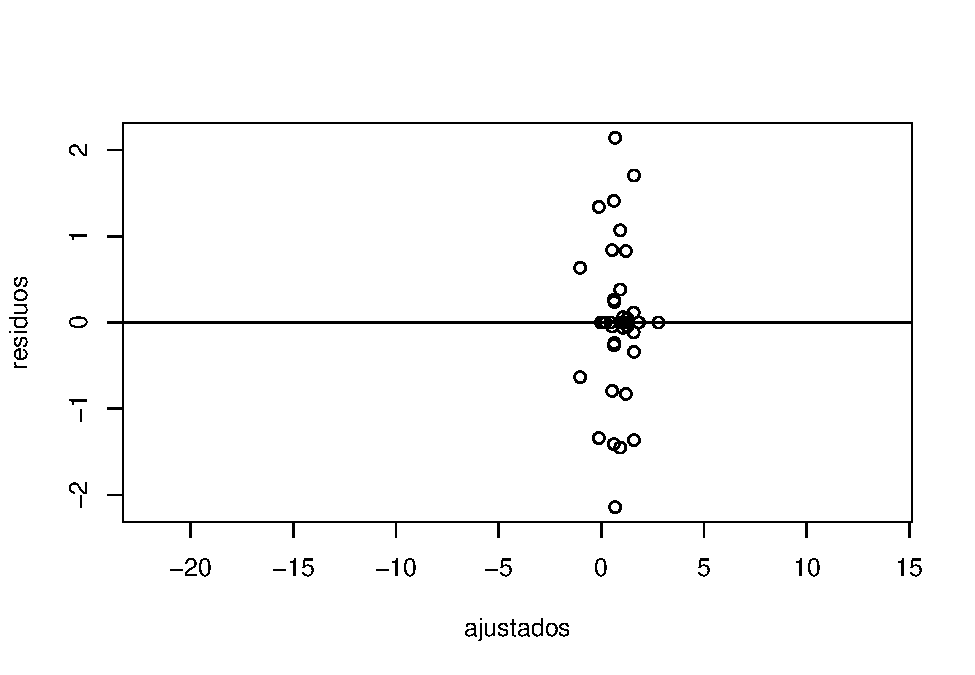
\includegraphics{Ejercicio-3_files/figure-latex/unnamed-chunk-15-1.pdf}
A continuación se muestran estos estadísticos:

\begin{longtable}[]{@{}clll@{}}
\toprule
\textbf{Coef.} & \textbf{Estimado} & \textbf{Std. Error} &
\textbf{T\_value} \\
\midrule
\endhead
intercepto & 4.300e01 & 00.802 & 0.536 \\
Y & 08.000 & 00.135 & 0.70 \\
R\^{}2 & 0.9882 & Adjusted R\^{}2 & 0.9168 \\
\bottomrule
\end{longtable}

Notemos que la \(R^2\) ajustada es muy alta, es decir, las variaciones
en el consumo se explican completamente por las variaciones en el
ingreso. Como ya mencionamos, este resultado indica que hay asociación
lineal entre las variables pues la \emph{bondad de ajuste} es mayor al
90\%.

\begin{enumerate}
\def\labelenumi{\arabic{enumi}.}
\setcounter{enumi}{2}
\tightlist
\item
  Ahora estimemos el tercer modelo de regresión lineal el cual está dado
  por la ecuación que sigue:
\end{enumerate}

\(\Delta_{C_t}=a+b\Delta_{Y_t-1}+\epsilon_t\)

Este modelo nos presenta una variable rezagada, es decir, lo que
buscamos analizar es si el ingreso afecta al consumo pero no en el mismo
periodo, es decir, queremos ver cómo afectan las variaciones en el
ingreso en \(t-1\) al consumo en \(t\).

Los resultados se muestran a continuación:

\(\Delta_{C_t}=+\Delta_{Y_t-1}\)

Los estadísticos se muestran en la siguiente tabla:

\begin{longtable}[]{@{}clll@{}}
\toprule
\textbf{Coef.} & \textbf{Estimado} & \textbf{Std. Error} &
\textbf{T\_value} \\
\midrule
\endhead
intercepto & 57.73 & 1.0857 & 48.57 \\
Y & 0.46927 & 0.01262 & 37.20 \\
R\^{}2 & 0.937 & Adjusted R\^{}2 & 0.9556 \\
\bottomrule
\end{longtable}

Notemos que la \(R^2\) ajustada es muy alta, es decir, las variaciones
en el consumo se explican completamente por las variaciones en el
ingreso. Como ya mencionamos, este resultado indica que hay asociación
lineal entre las variables pues la \emph{bondad de ajuste} es mayor al
90\%.

\begin{enumerate}
\def\labelenumi{\arabic{enumi}.}
\setcounter{enumi}{3}
\tightlist
\item
  Ahora estimemos el cuarto modelo de regresión lineal el cual está dado
  por la ecuación que sigue:
\end{enumerate}

\(ln(c_t)=a+bln(y_t)+\epsilon_t\)

Los resultados se muestran en la ecuación que sigue:

\(ln(c_t)=-14.27+1.13ln(y_t)+\epsilon_t\)

Es decir, que a cambios en \(Y_t\) el consumo responderá de forma
directa en un 1.13, lo que viene dado por el coeficiente \(b=1.13\).

Esta regresión se grafica en la siguiente tabla. Nótese que la relación
es directa y que el logaritmo del consumo está suficientemente explicado
por el logaritmo del ingreso.

Notemos que la propensión marginal a consumir es igual a 1.13, es decir,
que cambios en el logaritmo del ingreso se traducen más que
proporcionalmente a cambios en el logaritmo del consumo.

\begin{figure}
\centering
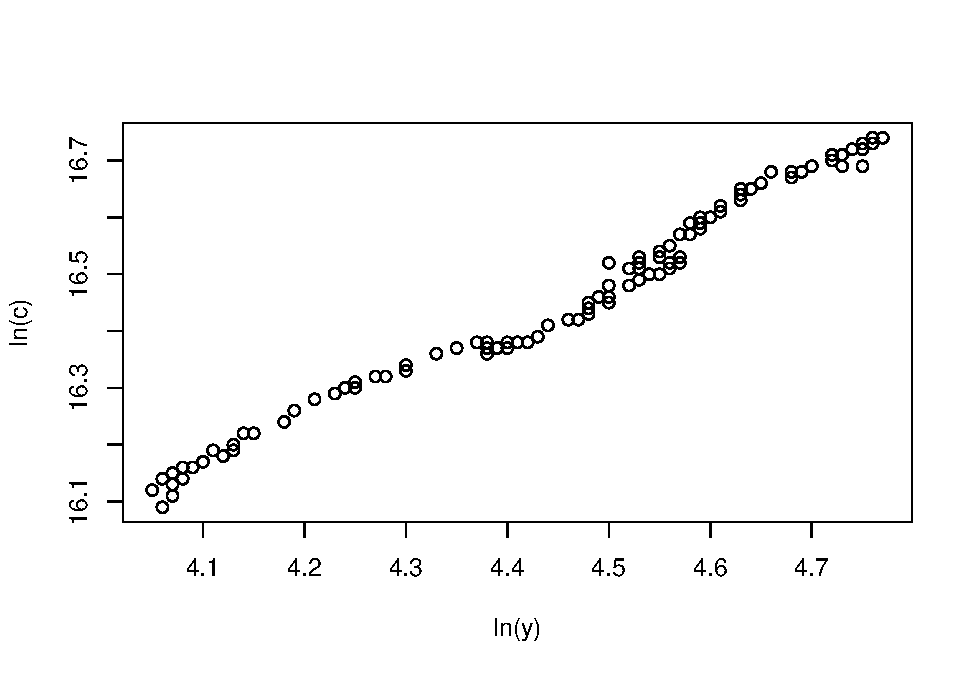
\includegraphics{Ejercicio-3_files/figure-latex/unnamed-chunk-17-1.pdf}
\caption{Modelo de regresión 4}
\end{figure}

Ahora notemos los errores. Eston están dados en la siguiente gráfica.
Notemos que estos errores presentan un patrón, lo que indica que hay
asociación lineal entre las variables. En el resumen de los estadísticos
de la regresión notaremos esta salvedad de la regresión:

\begin{figure}
\centering
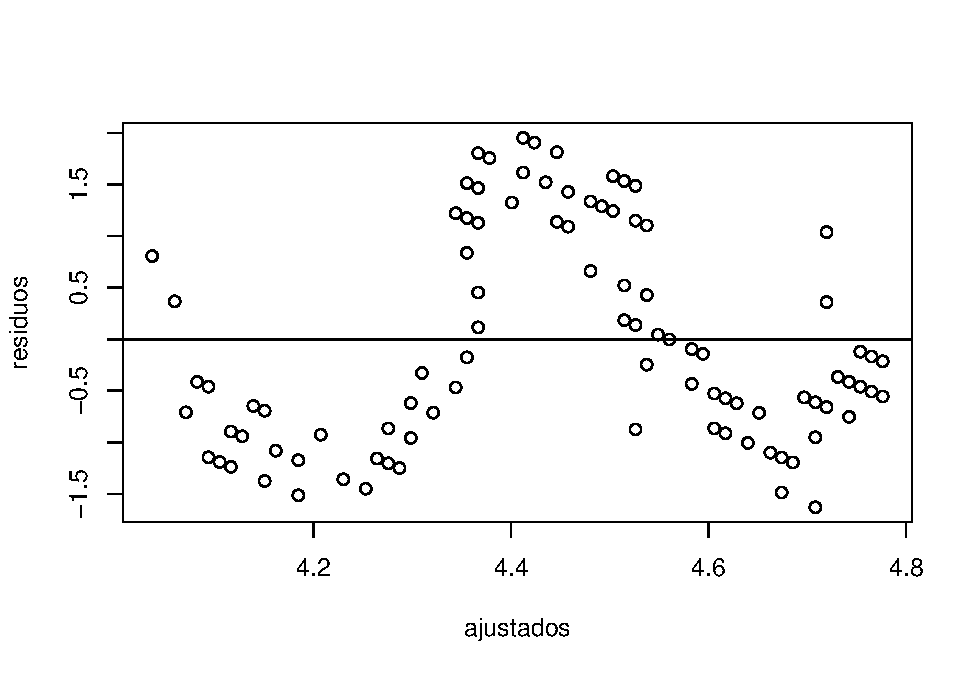
\includegraphics{Ejercicio-3_files/figure-latex/unnamed-chunk-18-1.pdf}
\caption{Errores: Modelo de regresión 4}
\end{figure}

La siguiente tabla muestra los resultados:

\begin{longtable}[]{@{}clll@{}}
\toprule
\textbf{Coef.} & \textbf{Estimado} & \textbf{Std. Error} &
\textbf{T\_value} \\
\midrule
\endhead
intercepto & -14.2753 & 0.2471 & -57.77 \\
Y & 1.1381 & 0.0150 & 75.87 \\
R\^{}2 & 0.9806 & Adjusted R\^{}2 & 0.9804 \\
\bottomrule
\end{longtable}

Notemos que la \(R^2\) ajustada es muy alta, es decir, que el logaritmo
del consumo se explica completamente por el logaritmo del ingreso. Como
ya mencionamos, este resultado indica que hay asociación lineal entre
las variables pues la \emph{bondad de ajuste} es cercana al 100\%. Por
tanto, los coeficientes calculados son no estadísticamente
significativos.

\hypertarget{g-explique-quuxe9-se-podruxeda-concluir-si-fuera-el-caso-acerca-de-la-hipuxf3tesis-de-ingreso-permanente-para-muxe9xico-a-partir-de-los-coeficientes-encontrados}{%
\subsubsection{g) Explique qué se podría concluir, si fuera el caso,
acerca de la Hipótesis de Ingreso Permanente para México a partir de los
coeficientes
encontrados}\label{g-explique-quuxe9-se-podruxeda-concluir-si-fuera-el-caso-acerca-de-la-hipuxf3tesis-de-ingreso-permanente-para-muxe9xico-a-partir-de-los-coeficientes-encontrados}}

A partir de todo el análisis hecho podemos concluir lo siguiente: i. Que
la HIP no explica el comportamiento del consumo agregado en la economía
mexicana para el periodo de observación. Este periodo abarca de 1993 a
2021, es decir, un periodo de 28 años. Esto implica que, a pesar de que
el consumo tiene un comportamiento poco volatil y con aumentos muy
cercanos a los aumentos del ingreso agregado, éste está determinado,
empíricamente, por las variaciones en el ingreso. De hecho, podemos
concluir que este efecto de sigue del efecto multiplicador Keynesiano
debido a que el consumo depende del ingreso y éste último también del
consumo, siendo el indicador importante \emph{la propensión marginal a
consumir}.

Esta propensión explica qué porcentajes de las variaciones en el ingreso
se traducen como variaciones directas en el consumo, y este
comportamiento se explica, esencialmente, por el modelo Keynesiano de
consumo. ii. No es posible eliminar la correlación que existe entre las
variables \(C_t\) y \(Y_t\) debido a la forma en la que se construyen.
No obstante, los modelos econométricos estimados nos confirman la
relación que teóricamente construimos entre las variables desde el
modelo lineal de consumo de la macroeconomía Keynesiana. Un análisis
econométrico más robusto excede el alcance de esta tarea, sin embargo,
es un área de oportunidad a explorar debido a que podríamos estimar con
mayor precisión cuál es la relación causal entre las variables y estimar
si es que las variaciones del ingreso, por ejemplo, impactan pero no
inmediatamente las variaciones en el consumo y hasta qué rezago se logra
absorber ese efecto.

Como conclusión, no es difícil demostrar que la HIP no se sostiene para
el caso de México, en el periodo observado, sin embargo, en línea con
las implicaciones empíricas expuestas en Romer, un análisis más robusto
implicaría identificar las variaciones del consumo que provienen de
variaciones permanentes o transitivas en el ingreso, por lo que esta
hipótesis no puede ser desechada completamente y más bien haría falta
hacer un análisis econométrico enfocado en clasificar las variaciones
transitivas y/o permanentes en el ingreso.

\end{document}
